\chapter{Implementierung}

\section{Atomare Maschinenbefehle}
Wie werden Sperren implementiert?

\subsubsection*{Naiver Versuch}
\begin{lstlisting}
belegen(l):
	Solange !l.frei gilt, wiederhole:    (1)
		warte einen Augenblick;          (2)
	setze l.frei = false;                (3)
\end{lstlisting}
Beispielablauf für 2 Threads, die versuchen, belegen(l) aufzurufen. Sei zu Beginn l.frei = true.
\begin{center}
\begin{tabular}{c c|c}
$P_1$ & $P_2$ & l.frei \\ \hline
(1) & \ & \ \\ 
\ & (1) & \ \\ 
(3) & \ & \ \\
\ & (3) & \ 
\end{tabular}
\end{center}
$\rightarrow$ Beide Threads sind im kritischen Bereich!\\
$\Rightarrow$ (1)(2)(3) muss selber wieder ein kritischer Bereich sein.\\
\\
Man benötigt einen speziellen Maschinenbefehl, z.B.:
\begin{lstlisting}
getAndSet(c, b, v):
	b := c;
	c := v;
\end{lstlisting}
Zwei Ausführungen dieses Maschinenbefehls müssen immer unter gegenseitigem Ausschlusds stattfinden, d.h. der Maschinenbefehl muss atomar (komplett und unteilbar) sein. Die Hardware muss dafür sorgen ("`Arbitrierung"').

\subsubsection*{Implementierung mit getAndSet}
\begin{lstlisting}
belegen(l):
	boolean b;
	getAndSet(l.frei, b, false);
	solange !b wiederhole:
		warte einen Augenblick;
		getAndSet(l.frei, b, false);

freigeben(l):
	boolean b;
	getAndSet(l.frei, b, true);
\end{lstlisting}

\subsubsection*{Alternativen}

\begin{lstlisting}
getAndInc(c, b):
	b := c;
	c := c + 1;
	
getAndDec(c, b):
	b := c;
	c := c - 1;

compareAndSet(c, e, v, b): // b := Wahrheitswert
	Falls c = e, dann:
		c := v;
		b := true;
	Sonst:
		b := false;
\end{lstlisting}
(Befehl CMPXCHG (compare exchange) auf Intel Pentium)

\subsubsection*{Implementierung mit compareAndSet}

\begin{lstlisting}
belegen(l):
	boolean b;
	compareAndSet(l.frei, true, false, b);
	Solange !b wiederhole:
		warte einen Augenblick;
		compareAndSet(l.frei, true, false, b);

freigeben(l):
	boolean b;
	compareAndSet(l.frei, false, true, b);
\end{lstlisting}

\textbf{Volatile} (engl. für flüchtig), Schlüsselwort in Java.\\
Beispiel:
\begin{lstlisting}
volatile int x;
\end{lstlisting}
x ist damit als gemeinsame Variable gekennzeichnet. Übliche Optimierungen des Compilers für lokale Variablen sind ausgeschlossen. Lese- und Schreibzugriffe auf x sind zueinander atomar ("`atomares Register"'). Die Hardware sorgt für Atomarität.

\section{Konsenszahlen}

n-Konsens mit \emph{compareAndSet} und \emph{get}:\\
(Einfaches Konsensproblem: Jeder schlägt sich selber vor)\\
\begin{lstlisting}
init(c):
    Setze c = -1.

entscheide(c, i, a): // mit i: Thread-ID des Aufrufers
    boolean b;
    compareAndSet(c, -1, i, b);
    Falls b gilt, dann:
        a := i;
    Sonst:
        a := get(c); // Kann auch ohne Fallunterscheidung
                     // angewandt werden, da fuer b true gilt:
                     // i == get(c)
\end{lstlisting}

\subsubsection*{Read/Modify/Write-Operation:}
rmw(c, b, f): (mit c ist gemeinsame Variable mit Wert vom Typ T, b ist Ergebnisvariable mit Wert von Typ T und f ist Modifikationsfunktion f: T $\rightarrow$ T).\\
b := c;\\
c := f(c);\\

Es gilt: \\
getAndSet(c, b, v) = rmw(c, b, $\lambda$x . v)\\
getAndInc(c, b) = rmw(c, b, $\lambda$x . x + 1)\\

Schar F von Funktionen von T nach T heißt \emph{Common2}, falls:

\begin{align}
	f(g(x)) & = f(x) \text{ (f absorbiert g) oder}\\
	g(f(x)) & = g(x) \text{ oder}\\
	f(g(x) & = g(f(x))	
\end{align}
für alle $f, g \in F, x \in T$ (trivial für f = g).\\
\\
F heißt \emph{nicht-trivial}, falls $ F \neq \{id\} $ mit $ F $ ist nichtleer, d.h. $ F \backslash \{id\} \neq \emptyset $.\\
\\
Beispiel: $ F = \{\lambda x\ .\ x + 1, \lambda x\ .\ x - 1\} = \{s, p\} $.\\
Es gilt: $ s(p(x) = x = p(s(x)) $ für alle $ x \in \mathbb{Z} $. Also ist $ F $ Common2. Damit Konsenszahl $\leq$ 2. Da $ F $ nicht-trivial, ist Konsenszahl = 2. 

\section{Zwischenspeicher}

\begin{description}
	\item[Zwischenspeicher (ZSP, engl. cache)] schneller, kleiner Speicher auf dem Prozessorchip.
\end{description}
Bemerkung: Herkunft des Begriffs "`cache"': Versteck der Beute eines Einbrechers.\\
\\
Verwendung:\\
Nachdem der Prozessor das erste Mal auf eine gewisse Arbeitsspeicherzelle lesend zugegriffen hat, speichert er den Wert in seinem ZSP. Wenn er das nächste Mal lesend auf dieselbe Adresse zugreifen will, findet er das Ergebnis in seinem ZSP ("`Treffer"', engl. match). Er braucht dazu nicht auf den BUS zuzugreifen.

Um schreibend auf eine Arbeitsspeicherzelle zuzugreifen, speichert der Prozessor das Wort zunächst in seinen ZSP. Nur wenn ein anderer Prozessor auf dieselbe Speicherzelle lesend zugreifen will, muss das Wort in den Arbeitsspeicher geschrieben werden.

\subsubsection*{Vorteil des ZSP:}
Weniger Zugriffe auf den Arbeitsspeicher nötig, damit schneller und der BUS ist weniger belastet.

Der ZSP lohnt sich, wenn im Programm häufig dicht hintereinander Zugriffe auf dieselbe Adresse vorkommen ("`Lokalität"').

Um den Verwaltungsaufwand gering zu halten, ist der ZSP in sogenannte \emph{Speicherzeilen} (engl. cache lines) organisiert. Sobald der ZSP voll ist, wird es nötig, manche Zeilen auszuwerfen (engl. to evict) um Platz zu schaffen.

\begin{description}
	\item[Kohärenz] Jeder Lesezugriff auf den ZSP liefert den zuletzt geschriebenen Wert.
\end{description}

Kohärenz bedeutet praktisch, dass sich durch die Einführung des ZSP nichts am Verhalten des Systems ändert.

Um Kohärenz zu erreichen, verwendet man ein Kohärenz-Protokoll, z.B. das MESI-Protokoll.

\subsubsection*{MESI-Protkoll:}

Jede Speicherzeile hat einen Modus:
\begin{description}
	\item[Modified] Zeile wurde verändert. Kein anderer Prozessor hat diese Zeile in seinem ZSP.
	\item[Exclusive] Zeile ist unverändert. Kein anderer Prozessor hat diese Zeile in seinem ZSP.
	\item[Shared] Zeile ist unverändert. Andere Prozessoren können diese Zeile in ihrem ZSP haben.
	\item[Invalid] Zeile enthält eine verwertbaren Daten.
\end{description}
Beispiel-Ablauf:\\
A, B, C seien Prozessoren, M sei ein Arbeitsspeicherblock.
\begin{figure}[H]
	\begin{center}
		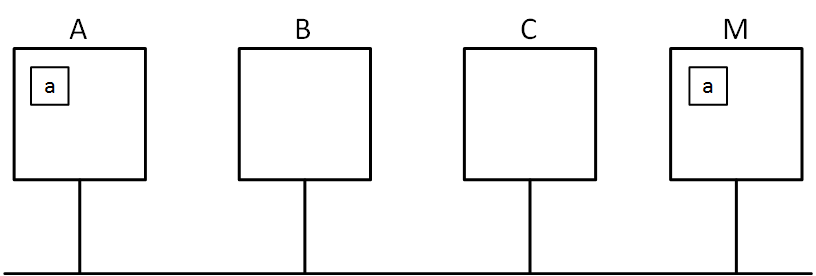
\includegraphics[width=.5\textwidth]{res/mesi_01}
		\caption{A liest Adresse von a.}
		\label{pic:mesi01}
	\end{center}
\end{figure} 
\begin{figure}[H]
	\begin{center}
		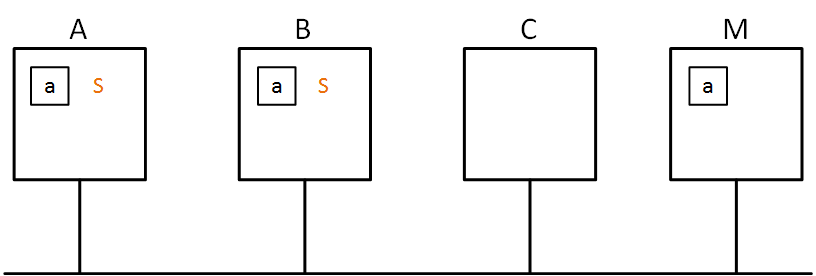
\includegraphics[width=.5\textwidth]{res/mesi_02}
		\caption{B liest Adresse von a; A antwortet.}
		\label{pic:mesi02}
	\end{center}
\end{figure} 
\begin{figure}[H]
	\begin{center}
		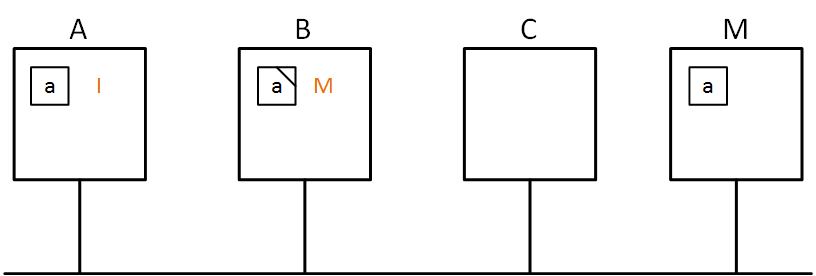
\includegraphics[width=.5\textwidth]{res/mesi_03}
		\caption{B schreibt auf Adresse a und informiert alle darüber.}
		\label{pic:mesi03}
	\end{center}
\end{figure} 
\begin{figure}[H]
	\begin{center}
		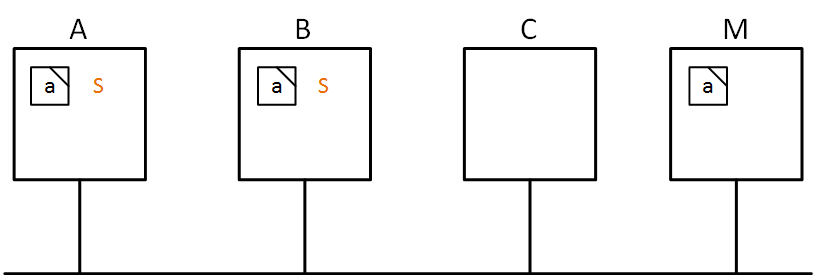
\includegraphics[width=.5\textwidth]{res/mesi_04}
		\caption{A liest von Adresse a, das führt zu Anfrage an alle, B sendet Daten.}
		\label{pic:mesi04}
	\end{center}
\end{figure} 

\begin{description}
	\item[False Sharing] gemeinsame Speicherzelle, obwohl sich die Daten darin nicht überlappen
\end{description}

Im ZSP von B:
\begin{figure}[H]
	\begin{center}
		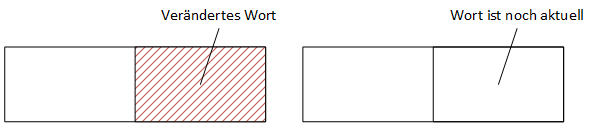
\includegraphics[width=.5\textwidth]{res/false_sharing_01}
		\caption{Speicherzeile für Adresse a.}
		\label{pic:falsesharing}
	\end{center}
\end{figure} 
False Sharing führt unnötig häufig zu Modus I.\\
\\
Daten, die nebeneinander verwendet werden, sollten in verschiedenen Speicherzeilen liegen.\\
\\
Verhalten mit getAndSet:\\
getAndSet(c, b, true)\\
Dabei ausgeführte Aktionen:
\begin{enumerate}
	\item c lesen
	\item b schreiben
	\item c schreiben
\end{enumerate}
\begin{figure}[H]
	\begin{center}
		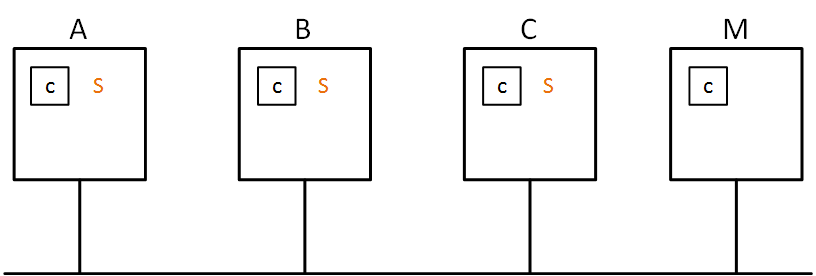
\includegraphics[width=.5\textwidth]{res/mesi_05}
		\caption{Zustand vorher.}
		\label{pic:mesi05}
	\end{center}
\end{figure} 
\begin{figure}[H]
	\begin{center}
		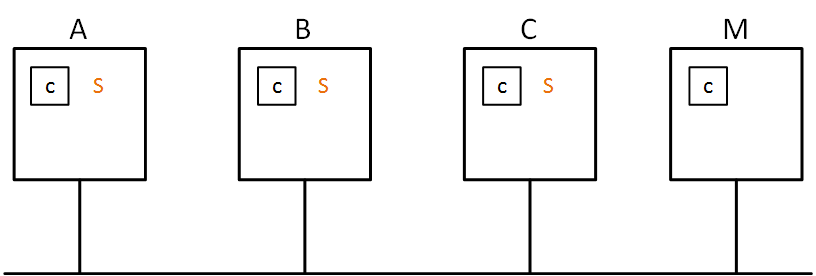
\includegraphics[width=.5\textwidth]{res/mesi_06}
		\caption{A führt (1) aus, Wert von c in ZSP von A ist bereits aktuell, keine Änderung.}
		\label{pic:mesi06}
	\end{center}
\end{figure} 
\begin{figure}[H]
	\begin{center}
		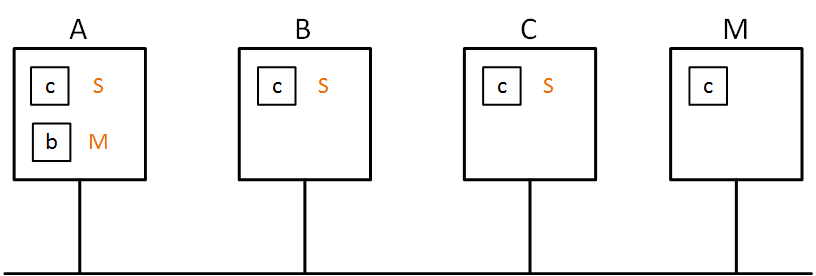
\includegraphics[width=.5\textwidth]{res/mesi_07}
		\caption{A führt (2) aus.}
		\label{pic:mesi07}
	\end{center}
\end{figure} 
\begin{figure}[H]
	\begin{center}
		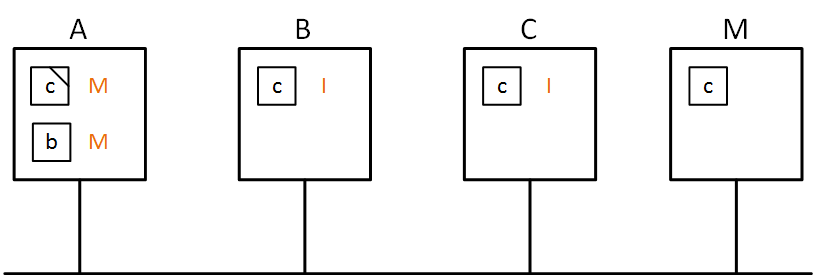
\includegraphics[width=.5\textwidth]{res/mesi_08}
		\caption{A führt (3) aus.}
		\label{pic:mesi08}
	\end{center}
\end{figure} 
\begin{figure}[H]
	\begin{center}
		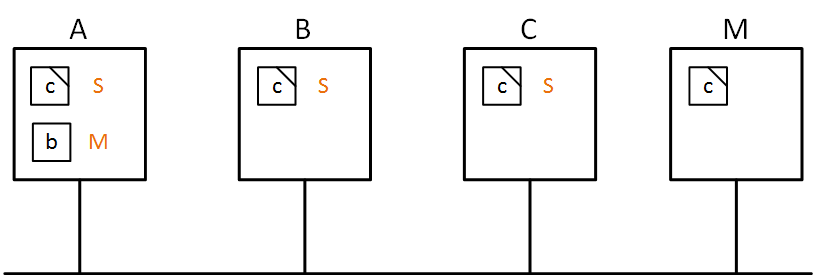
\includegraphics[width=.5\textwidth]{res/mesi_09}
		\caption{B führt (1) aus.}
		\label{pic:mesi09}
	\end{center}
\end{figure} 
\begin{figure}[H]
	\begin{center}
		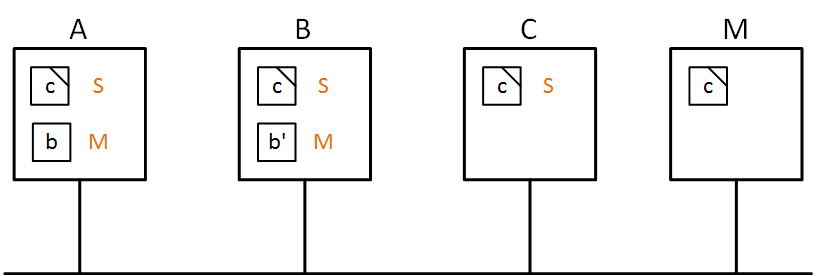
\includegraphics[width=.5\textwidth]{res/mesi_10}
		\caption{B führt (2) aus.}
		\label{pic:mesi10}
	\end{center}
\end{figure} 
\begin{figure}[H]
	\begin{center}
		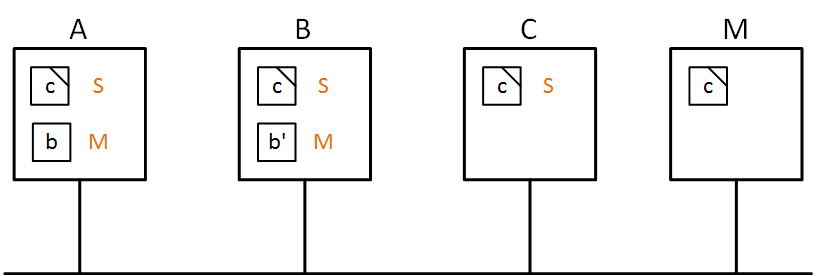
\includegraphics[width=.5\textwidth]{res/mesi_11}
		\caption{B führt (3) aus, keine Änderung, denn der Wert in c verändert sich nicht dabei.}
		\label{pic:mesi11}
	\end{center}
\end{figure} 

Alle getAndSet-Aufrufe der Warteschleife können ohne BUS-Zugriff abgearbeitet werden.

\section{Bäckerei-Algorithmus}
\begin{description}
	\item[Bäckerei-Algorithmus (engl bakery algorithm)] von Leslie Lamport 1974 publiziert; Implementierung von Sperren mit atomaren Registern.
\end{description}

Analogie: Jeder, der (in Amerika) eine Bäckerei betritt, zieht zuerst eine laufende Nummer. Der Kunde mit der niedrigsten Nummer wird als nächste bedient.\\
\\
Pseudocode mit einer Sperre:\\
\begin{lstlisting}[escapeinside={(*}{*)}]
Typ Thread ID = {0, ..., n - 1}; // n Threads
volatile flag: boolean[ThreadID]; // initialisiert mit false
volatile label: long[ThreadID]; // initialisiert mit 0
Prozedur belegen():
    int i := Nummer des aufrufenden Threads;
    flag[i] := true;
    label[i] := max(label[0], ..., label[n - 1]) + 1;
    Warte solange (* $\exists k \neq i : \text{flag}[k] \land \left(\text{label}[k], k\right) <_\text{lex} \left(\text{label}[i], i\right)$ *)
Prozedur freigeben():
    flag[Nummer des aufrufenden Threads] := false;
\end{lstlisting}
\textbf{Behauptung:} Der Bäckerei-Algorithmus hat die Fortschritt-Eigenschaft.\\
\textbf{Beweis:} Der Thread i mit dem kleinsten Paar (label[i], i) wartet nicht. Es gibt so ein i, denn $<_\text{lex}$ ist eine Wohlordnung. Damit hat jede nicht-leere Menge ein kleinstes Element.\\
\\
\textbf{Behauptung:} Der Bäckerei-Algorithmus ist FCFS (First Come First Serve).\\
\textbf{Beweis:} Falls Thread i den Torweg verlässt, bevor Thread j ihn betritt, dann gilt:
\begin{align*}
	& w_i\left(label[i], v\right) \rightarrow\\
	& r_j\left(label[i], v\right) \rightarrow\\
	& w_j\left(label[j], v'\right) \text{ mit } v < v'\\
	& r_j\left(flag[i], true\right)
\end{align*}
Dabei bedeutet $w_i\left(label[i], v\right)$: Schreibzugriff von Thread $i$ auf die Variable $label[i]$; der geschriebene Wert ist v.\\
Es gilt $flag[i] \land \left(flat[i], i\right) <_\text{lex} \left(label[j], j\right)$.\\
Aus Fortschritt und FCFS folgt Fairness.\\
\\
\textbf{Behauptung:} Der Bäckerei-Algorithmus erfüllt gegenseitigen Ausschluss.\\
\textbf{Beweis:} Durch Widerspruch (grundsätzliche Methode: Man behauptet, zwei Threads seien simulatan im kritischen Bereich. Herbeiführung von Widerspruch). Angenommen Threads i und j sind nebeneinander im kritischen Bereich. O.B.d.A. gilt: $\left(label[i], i\right) <_\text{lex} \left(label[j], j\right)$. Sobald Thread j die Warteschleife verlassen hat, gilt:
\begin{equation*}
	flag[i] = false \text{ (1)}
\end{equation*}
oder
\begin{equation*}
	\left(label[j], j\right) <_\text{lex} \left(label[i], i\right) \text{ (2)}
\end{equation*}
Die Werte von i und j sind fest. Der Wert von label[j] ändert sich nicht mehr bis zum Betreten des kritischen Bereichs. Der Wert von label[i] kann höchstens größer werden.\\
Wenn also (2) beim Verlassen der Warteschleife gilt, dann auch im kritischen Bereich. Widerspruch!\\
Also gilt (1). Deswegen 
\begin{align*}
&	r_j\left(\text{label}[i], \_\right) \rightarrow \text{ (\_: gelesener Wert ist irrelevant)}\\
&	w_j\left(\text{label}[j], v\right) \rightarrow\\
&	r_j\left(\text{flag}[i], false\right) \rightarrow\\
&	w_i\left(\text{flag}[i], true\right) \rightarrow\\
&	r_i\left(\text{label}[j], v\right) \rightarrow\\
&	w_i\left(\text{label}[i], v'\right)
\end{align*}
mit $v < v'$, also $\text{label}[j] < \text{label}[i]$. Widerspruch!\\
\\
Nachteil: Falls nur atomare Lese- und Schreib-Operationen zur Verfügung stehen ("`atomare Register"'), sind für n Threads Lese- und Schreibzugriffe auf mindestens n Speicherzellen notwendig (Burns/Lynch 1993).\\
Grund: Jeder Thread benötigt eine Speicherzelle, auf die nur er schreibt. Sonst kann ein anderer Thread das überschreiben, was ein anderer geschrieben hat.\\
Es muss mindestens n + 1 unterscheidbare Zustände geben: 
\begin{enumerate}
	\item kein Thread befindet sich im kritischen Bereich
	\item Thread i befindet sich im kritischen Bereich
\end{enumerate}